%%--------------------------------------------------------
%% example.tex
%%
%%--------------------------------------------------------
\documentclass[12pt]{article}

%%%%%%%%%%%%%%%%%%%%%%%%%%%%%%%%%%%%%%%%%%%%%%%%%%%%%%%%%%%%%%%%%%
%%% Comment out to use biblatex instead of bibtex
%%%%%%%%%%%%%%%%%%%%%%%%%%%%%%%%%%%%%%%%%%%%%%%%%%%%%%%%%%%%%%%%%%
\def\UseBibLatex{1}

%%%%%%%%%%%%%%%%%%%%%%%%%%%%%%%%%%%%%%%%%%%%%%%%%%%%%%%%%%%%%%%%%
% Put all your private style files/class style files in the styles/
% subdirectory. The following command guarantee that latex would find
% it.
%%%%%%%%%%%%%%%%%%%%%%%%%%%%%%%%%%%%%%%%%%%%%%%%%%%%%%%%%%%%%%%%%

\makeatletter
\def\input@path{{styles/}}
\makeatother


%%%%%%%%%%%%%%%%%%%%%%%%%%%%%%%%%%%%%%%%%%%%%%%%%%%%%%%%%%%%%%%%%%
% A modified usepackge command that checks for style files in the
% styles/ subdirectory.
%%%%%%%%%%%%%%%%%%%%%%%%%%%%%%%%%%%%%%%%%%%%%%%%%%%%%%%%%%%%%%%%%% 
\newcommand{\UsePackage}[1]{%
  \IfFileExists{styles/#1.sty}{%
      \usepackage{styles/#1}%
   }{%
      \IfFileExists{../styles/#1.sty}{%
         \usepackage{../styles/#1}%
      }{%
         \usepackage{#1}%
      }%
   }%
}


\usepackage[T1]{fontenc}
\usepackage{lmodern}
\usepackage{textcomp}

\usepackage{amsmath}%
\usepackage{amssymb}%
\usepackage[table]{xcolor}%

\setlength{\marginparwidth}{6cm} 
\usepackage{todonotes}
\usepackage[in]{fullpage}%

\usepackage[amsmath,thmmarks]{ntheorem}%
\theoremseparator{.}%

\usepackage{titlesec}%
\titlelabel{\thetitle. }%
\usepackage{xcolor}%
\usepackage{mleftright}%
\usepackage{xspace}%
\usepackage{graphicx}
\usepackage{hyperref}%

\newcommand{\hrefb}[3][black]{\href{#2}{\color{#1}{#3}}}%

\usepackage{hyperref}%
\hypersetup{%
      unicode,
      breaklinks,%
      colorlinks=true,%
      urlcolor=[rgb]{0.25,0.0,0.0},%
      linkcolor=[rgb]{0.5,0.0,0.0},%
      citecolor=[rgb]{0,0.2,0.445},%
      filecolor=[rgb]{0,0,0.4},
      anchorcolor=[rgb]={0.0,0.1,0.2}%
}
\usepackage[ocgcolorlinks]{ocgx2}

%%%%%%%%%%%%%%%%%%%%%%%%%%%%%%%%%%%%%%%%%%%%%%%%%%%%%%%%%%%%%%%%%%%%%%%%
% Defining theorem like environments
%

\theoremseparator{.}%

\theoremstyle{plain}%
\newtheorem{theorem}{Theorem}[section]

\newtheorem{lemma}[theorem]{Lemma}
\newtheorem{conjecture}[theorem]{Conjecture}
\newtheorem{corollary}[theorem]{Corollary}
\newtheorem{claim}[theorem]{Claim}%
\newtheorem{fact}[theorem]{Fact}
\newtheorem{observation}[theorem]{Observation}
\newtheorem{invariant}[theorem]{Invariant}
\newtheorem{question}[theorem]{Question}
\newtheorem{proposition}[theorem]{Proposition}
\newtheorem{prop}[theorem]{Proposition}
\newtheorem{openproblem}[theorem]{Open Problem}

\theoremstyle{plain}%
\theoremheaderfont{\sf} \theorembodyfont{\upshape}%
\newtheorem*{remark:unnumbered}[theorem]{Remark}%
\newtheorem*{remarks}[theorem]{Remarks}%
\newtheorem{remark}[theorem]{Remark}%
\newtheorem{definition}[theorem]{Definition}
\newtheorem{defn}[theorem]{Definition}
\newtheorem{example}[theorem]{Example}
\newtheorem{exercise}[theorem]{Exercise}
\newtheorem{problem}[theorem]{Problem}
\newtheorem{xca}[theorem]{Exercise}
\newtheorem{exercise_h}[theorem]{Exercise}
\newtheorem{assumption}[theorem]{Assumption}%

% Proof environment
\newcommand{\myqedsymbol}{\rule{2mm}{2mm}}

\theoremheaderfont{\em}%
\theorembodyfont{\upshape}%
\theoremstyle{nonumberplain}%
\theoremseparator{}%
\theoremsymbol{\myqedsymbol}%
\newtheorem{proof}{Proof:}%

\newtheorem{proofof}{Proof of\!}%

% theorem block end
%%%%%%%%%%%%%%%%%%%%%%%%%%%%%%%%%%%%%%%%%%%%%%%%%%%%%%%%%%%%%%%%%%%%


%%%%%%%%%%%%%%%%%%%%%%%%%%%%%%%%%%%%%%%%%%%%%%%%%%%%%%%%%%%%%%%%%% 5
% Color emph

\providecommand{\emphind}[1]{}%
\renewcommand{\emphind}[1]{\emph{#1}\index{#1}}

\definecolor{blue25emph}{rgb}{0, 0, 11}

\providecommand{\emphic}[2]{}
\renewcommand{\emphic}[2]{\textcolor{blue25emph}{%
      \textbf{\emph{#1}}}\index{#2}}

\providecommand{\emphi}[1]{}%
\renewcommand{\emphi}[1]{\emphic{#1}{#1}}

\definecolor{almostblack}{rgb}{0, 0, 0.3}

\providecommand{\emphw}[1]{}%
\renewcommand{\emphw}[1]{{\textcolor{almostblack}{\emph{#1}}}}%

\providecommand{\emphOnly}[1]{}%
\renewcommand{\emphOnly}[1]{\emph{\textcolor{blue25}{\textbf{#1}}}}

% Color emph - end
%%%%%%%%%%%%%%%%%%%%%%%%%%%%%%%%%%%%%%%%%%%%%%%%%%%%%%%%%%%%%%%%%% 5

%%%%%%%%%%%%%%%%%%%%%%%%%%%%%%%%%%%%%%%%%%%%%%%%%%%%%%%%%%%%%%%%%%%
% Authors thanks
%%%%%%%%%%%%%%%%%%%%%%%%%%%%%%%%%%%%%%%%%%%%%%%%%%%%%%%%%%%%%%%%%%%

\newcommand{\JamesThanks}[1]{%
   \thanks{%
      Department of Computer Science; %
      University of Moochi; %
      102 S. Bad St; %
      Blackstone, SF, 12345, USA; %
      \href{mailto:spam@spam.edu}{spam@spam.edu}; %
      \url{http://spammer.org/}. %
   #1%
   }%
}

%%%%%%%%%%%%%%%%%%%%%%%%%%%%%%%%%%%%%%%%%%%%%%%%%
\newcommand{\james}[1]{%   
\todo[author=James,inline,color=blue!25]{#1}}
\newcommand{\ford}[1]{%   
\todo[author=Ford,inline,color=red!25]{#1}}


%%%%%%%%%%%%%%%%%%%%%%%%%%%%%%%%%%%%%%%%%%%%%%%%%%%%%%%%%%%%%%%%%%%%%%
%    Handling references
%%%%%%%%%%%%%%%%%%%%%%%%%%%%%%%%%%%%%%%%%%%%%%%%%%%%%%%%%%%%%%%%%%%%%%

\newcommand{\HLink}[2]{\hyperref[#2]{#1~\ref*{#2}}}
\newcommand{\HLinkSuffix}[3]{\hyperref[#2]{#1\ref*{#2}{#3}}}

\newcommand{\figlab}[1]{\label{fig:#1}}
\newcommand{\figref}[1]{\HLink{Figure}{fig:#1}}

\newcommand{\thmlab}[1]{{\label{theo:#1}}}
\newcommand{\thmref}[1]{\HLink{Theorem}{theo:#1}}

\newcommand{\remlab}[1]{\label{rem:#1}}
\newcommand{\remref}[1]{\HLink{Remark}{rem:#1}}%

\newcommand{\corlab}[1]{\label{cor:#1}}
\newcommand{\corref}[1]{\HLink{Corollary}{cor:#1}}%

\providecommand{\deflab}[1]{}
\renewcommand{\deflab}[1]{\label{def:#1}}
\newcommand{\defref}[1]{\HLink{Definition}{def:#1}}

\newcommand{\lemlab}[1]{\label{lemma:#1}}
\newcommand{\lemref}[1]{\HLink{Lemma}{lemma:#1}}%

\providecommand{\eqlab}[1]{}%
\renewcommand{\eqlab}[1]{\label{equation:#1}}
\newcommand{\Eqref}[1]{\HLinkSuffix{Eq.~(}{equation:#1}{)}}

%%%%%%%%%%%%%%%%%%%%%%%%%%%%%%%%%%%%%%%%%%%%%%%%%%%%%%%%%%%%%%%%%%%

\newcommand{\remove}[1]{}%
\newcommand{\Set}[2]{\left\{ #1 \;\middle\vert\; #2 \right\}}

\newcommand{\pth}[1]{\mleft(#1\mright)}%

\newcommand{\ProbC}{{\mathbb{P}}}
\newcommand{\ExC}{{\mathbb{E}}}
\newcommand{\VarC}{{\mathbb{V}}}

\newcommand{\Prob}[1]{\ProbC\mleft[ #1 \mright]}
\newcommand{\Ex}[1]{\ExC\mleft[ #1 \mright]}
\newcommand{\Var}[1]{\VarC\mleft[ #1 \mright]}


\newcommand{\ceil}[1]{\mleft\lceil {#1} \mright\rceil}
\newcommand{\floor}[1]{\mleft\lfloor {#1} \mright\rfloor}

\newcommand{\brc}[1]{\left\{ {#1} \right\}}
\newcommand{\set}[1]{\brc{#1}}%

\newcommand{\cardin}[1]{\left\lvert {#1} \right\rvert}%

\renewcommand{\th}{th\xspace}
\newcommand{\ds}{\displaystyle}%

\renewcommand{\Re}{\mathbb{R}}%
\newcommand{\reals}{\Re}%


%%%%%%%%%%%%%%%%%%%%%%%%%%%%%%%%%%%%%%%%%%%%%%%%%%%%%%%%%%%%%%%%%%%%%%%%%
% Defining comptenum environment using enumitem
\usepackage[inline]{enumitem}

\newlist{compactenumA}{enumerate}{5}%
\setlist[compactenumA]{topsep=0pt,itemsep=-1ex,partopsep=1ex,parsep=1ex,%
   label=(\Alph*)}%

\newlist{compactenuma}{enumerate}{5}%
\setlist[compactenuma]{topsep=0pt,itemsep=-1ex,partopsep=1ex,parsep=1ex,%
   label=(\alph*)}%

\newlist{compactenumI}{enumerate}{5}%
\setlist[compactenumI]{topsep=0pt,itemsep=-1ex,partopsep=1ex,parsep=1ex,%
   label=(\Roman*)}%

\newlist{compactenumi}{enumerate}{5}%
\setlist[compactenumi]{topsep=0pt,itemsep=-1ex,partopsep=1ex,parsep=1ex,%
   label=(\roman*)}%

\newlist{compactitem}{itemize}{5}%
\setlist[compactitem]{topsep=0pt,itemsep=-1ex,partopsep=1ex,parsep=1ex,%
   label=\ensuremath{\bullet}}%


%%%%%%%%%%%%%%%%%%%%%%%%%%%%%%%%%%%%%%%%%%%%%%%%%%%%%%%%%%%%%%%%%%%%%%%%%%

%%%%%%%%%%%%%%%%%%%%%%%%%%%%%%%%%%%%%%%%%%%%%%%%%%%%%%%%%%%%%%%%%%%
% Biblatex....
%
\providecommand{\BibLatexMode}[1]{}
\providecommand{\BibTexMode}[1]{}

\ifx\UseBibLatex\undefined%
  \renewcommand{\BibLatexMode}[1]{}
  \renewcommand{\BibTexMode}[1]{#1}
\else
  \renewcommand{\BibLatexMode}[1]{#1}
  \renewcommand{\BibTexMode}[1]{}
\fi


% Bib latex stuff
\BibLatexMode{%
   \usepackage[bibencoding=utf8,style=alphabetic,backend=biber]{biblatex}%
   \UsePackage{my_biblatex}%
}

%
%%%%%%%%%%%%%%%%%%%%%%%%%%%%%%%%%%%%%%%%%%%%%%%%%%%%%%%%%%%%%%%%%%%

\numberwithin{figure}{section}%
\numberwithin{table}{section}%
\numberwithin{equation}{section}%



%%%%%%%%%%%%%%%%%%%%%%%%%%%%%%%%%%%%%%%%%%%%%%%%%%%%%%%%%%%%%%%%%%%
%%%%%%%%%%%%%%%%%%%%%%%%%%%%%%%%%%%%%%%%%%%%%%%%%%%%%%%%%%%%%%%%%%%
% Papers specific commands...
%%%%%%%%%%%%%%%%%%%%%%%%%%%%%%%%%%%%%%%%%%%%%%%%%%%%%%%%
%%%%%%%%%%%%%%%%%%%%%%%%%%%%%%%%%%%%%%%%%%%%%%%%%%%%%%%%



%%%%%%%%%%%%%%%%%%%%%%%%%%%%%%%%%%%%%%%%%%%%%%%%%%%%%%%%
%%BeginIpePreamble
%%%%%%%%%%%%%%%%%%%%%%%%%%%%%%%%%%%%%%%%%%%%%%%%%%%%%%%%


%%%%%%%%%%%%%%%%%%%%%%%%%%%%%%%%%%%%%%%%%%%%%%%%%%%%%%%%
%%EndIpePreamble
%%%%%%%%%%%%%%%%%%%%%%%%%%%%%%%%%%%%%%%%%%%%%%%%%%%%%%%%
%

\BibLatexMode{%
   \bibliography{template}
}
\usepackage{float}
\usepackage{verbatim}
\begin{document}

\title{What makes a great Agent?}

\author{%
   James Bond%
   \JamesThanks{Bla bla.}%
   %
   \and%
   %
   Ford Perfect%
   \thanks{Bla bla.}%
}

\date{\today}

\maketitle

\begin{abstract}
    %%% DELETE START
    Role play, focus, tools, cooperation, guardrails, memory.
    core concept, using tool at scale, tasks and processes, agentic collaboration, build a complete crew
    %%% DELETE END
\end{abstract}


%%%%%%%%%%%%%%%%%%%%%%%%%%%%%%%%%%%%%%%%%%%%%%%%%%%%%%
%%%%%%%%%%%%%%%%%%%%%%%%%%%%%%%%%%%%%%%%%%%%%%%%%%%%%%

\section{AI Agents}

%%% DELETE START 

%%%%%%%%%%%%%%%%%%%%%%%%%%%%%%%%%%%%%%%%%%%%%%%%
%%% TO USE TEMPLATE DELETE EVERYTHING FROM HERE...


% All the \LaTeX{} definitions/macros/etc are in the \texttt{prefix.tex} file. This makes this file a bit cleaner.
Agents, Tasks, crews

-task-> tools, answer
- Agent -> task -> crew


\begin{figure}[H]
    \centering
    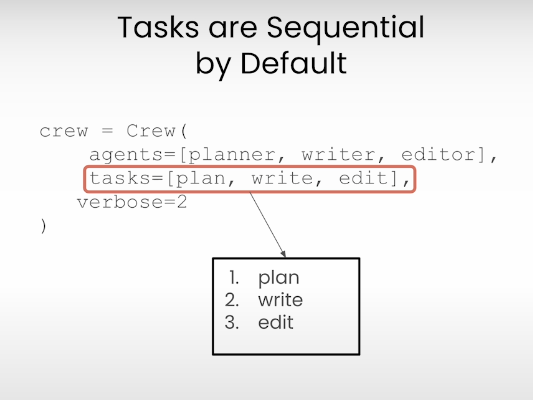
\includegraphics{images/agents_tasks_crews_diagram.png}
    \caption{agents tasks crews diagram}
    \label{fig:agents_tasks_crews_diagram}
\end{figure}
%%%end figure
\begin{theorem}
    \thmlab{first}%
    %
    Bla bla.
\end{theorem}
\begin{proof}
    This is the proof.
    \[
    \sqrt{2} + \sqrt{2} = 2 \sqrt{2}.
    \]
\end{proof}

\james{It is extremely useful to leave comments in the text for your coauthors.}
\ford{And the other author might reply...}
\james{But one can still have the last word. }

See \thmref{first}.
\begin{lemma}
    \lemlab{second}.
    %
    This is a lemma.
\end{lemma}

See \lemref{second}.

\begin{definition}
    \deflab{number}
    A number is a \emphi{number}.
\end{definition}

See also \defref{number}.

\begin{remark}
    \remlab{useful}
    Remarks are useful sometime.
\end{remark}

Was \remref{useful} useful?

\section{Multi agent customer support automation}
\begin{verbatim}
crew = Crew(
  agents=[support_agent, support_quality_assurance_agent],
  tasks=[inquiry_resolution, quality_assurance_review],
  verbose=2,
  memory=True
)
\end{verbatim}

Do not forget to cite some irrelevant papers \cite{k-spda-10}.

%------------------------------------------------------------------
%------------------------------------------------------------------

\section{Mental framwork for agent creation}
Some math:
\begin{equation*}
    \Var{X}%
    =%
    \Ex{(X - \Ex{X})^2}.
\end{equation*}

Some definitions.
\begin{defn}
    \deflab{prime}%
    %
    An integer number $p > 1$ is \emphi{prime} if it is divisible
    only by $1$ or itself.
\end{defn}

A theorem:
\begin{theorem}
    \thmlab{main}% Label for the theorm
    %
    The number of primes is unbounded.
\end{theorem}
\begin{proof}
    Assume for the sake of contradiction that the number of primes is
    finite, say $k$, and let $1 < p_1< p_2 < \cdots < p_k$ be these
    primes. Observe that $N = p_1 \cdot p_2 \cdots p_k +1 > 1$ is
    indivisible by $p_1, \ldots, p_k$, and is larger than all these
    numbers. Thus, $N$ must be prime. A contradiction.
\end{proof}

\defref{prime} and \thmref{main} were both known to the Greeks. Well,
to some of the Greeks.

\bigskip

I prefer to use \texttt{enumitem} for creating lists:
\begin{compactenumI}
    \smallskip%
    \item One can create more compact lists.

    \smallskip%
    \item There is more control over labels.
\end{compactenumI}
\smallskip%
And another good reason is because:
\begin{compactenumI}[resume]
    \smallskip%
    \item One can resume the numbering.
\end{compactenumI}

\bigskip%

It is usually a good idea to let \LaTeX{} do its thing. Do not use
\textbackslash\textbackslash{} to end lines (common mistakes for
\LaTeX{} beginners). End a paragraph by having an empty line. If you
want a big space between two paragraphs, just put
\texttt{\textbackslash{big{}skip}} in a line on its own between th two
paragraphs.

\bigskip

Just like that.


\paragraph{Paragraphs.}

I like to title my paragraphs so that people know what the paragraph
is about. This is a personal style thing, as area lot of other writing
stuff. Follow what you like. More sectioning commands follow. If you
comment out the
\texttt{\textbackslash{}def\textbackslash{}UseBibLatex{1}} then the
system would use bibtex instead.

\subsection{A subsection}

\subsection{A lemma example}

\begin{lemma}
    This is a lemma.
\end{lemma}


%------------------------------------------------------------------
%------------------------------------------------------------------

\section{Bibliography}

Nowadays, I like to use \texttt{biblatex}, but it is somewhat more
painful to use than \texttt{bibtex}. The big advantage of
\texttt{biblatex} that it is highly configurable if you are willing to
spend the energy to learn it. It does much better work than
\texttt{bibtex}. I highly recommend getting your bibtex entry from
DBLP, since they have the \texttt{doi} information -- this implies
that you get a link to the paper in \texttt{biblatex} or
\texttt{bibtex} if you use the right style.

Anyway, here is an example of a citation \cite{k-spda-10}.





%%% DELETE END

\section*{Acknowledgments}

%%% DELETE START
Thank everyone.
%%% DELETE END

%-------------------------------------------------------------------------

\BibTexMode{%
   \bibliographystyle{alpha}
   \bibliography{template}
}%
\BibLatexMode{\printbibliography}

\end{document}


%--------------------------------------------------------
%
% x.tex - end of file
%--------------------------------------------------------
